%\documentclass[draft]{ws-procs9x6}
\documentclass{ws-procs9x6}
\usepackage{comment}
\usepackage{subfigure}
\usepackage{color}

\begin{document}

\title{Bridging the gap: improving local multiple alignment with a novel heuristic for gapped extension.}

\author{Todd J. Treangen$^\dag*$}

\address{Dept. of Computer Science, Technical Univ. of Catalonia\\
Barcelona, Spain\\
$^*$E-mail: treangen@lsi.upc.edu}

\author{Aaron E. Darling$^\dag*$}

\address{Institute for Molecular Bioscience, Univ. of Queensland\\
Brisbane, Australia\\
$^*$E-mail: a.darling@imb.uq.edu.au}


\author{Guillaume Achaz}

\address{Atelier de Bioinformatique, Univ. Pierre et Marie Curie-Paris 6\\
Paris, France}

\author{ Mark A. Ragan}

\address{Institute for Molecular Bioscience, Univ. of Queensland\\
Brisbane, Australia\\
}

\author{ Xavier Messeguer}

\address{Dept. of Computer Science, Technical Univ. of Catalonia\\
Barcelona, Spain\\
}

{\center \scriptsize $^\dag$ These authors contributed equally to this work \\}

\begin{abstract}
The identification of homologous DNA via sequence alignment is a basic building block in comparative genomics.  We present a method for accurately and sensitively identifying homologous DNA sequence in multiple genomes. Our method is based around an efficient heuristic for local multiple alignment, featuring a novel method for gapped extensions. In practice, we are able to sensitively identify conserved, potentially repetitive, regions in one or more DNA sequences.
\end{abstract}

\keywords{sequence alignment}


\bodymatter

\section{Introduction}

The importance of accurate homology identification to comparative genomics can not be overestimated~\cite{Kumar07}. To date, pairwise local sequence alignment methods~\cite{ref-blastz, ref-ssearch,repseek} have been the prevailing technique to identify homologous nucleotides.  When more than two copies of a homologous sequence element are present in the data, pairwise homology detection methods generate a listing of all possible pairs of homologous elements.  Apart from the obvious inefficiency of considering all pairwise homology relationships, a collection of pairwise alignments is not ideal because they are rarely amenable to comparative genomic and phylogenetic analysis without further processing into a multiple alignment.

Local pairwise alignments can be merged to create a multiple alignment by a variety of methods~\cite{ref-tba,ref-aba,ref-dialign,ref-related1}. Such methods commonly assume that pairwise homology relationships are transitive, such that if nucleotide $a$ is homologous to nucleotide $b$, and $b$ is to $c$, then $a$ must also be homologous to $c$.  Thus, in order to merge pairwise alignments, such methods must tackle the challenging problem of resolving inconsistent transitive homology relationships.  Pairwise alignment has been demonstrated to be less accurate than multiple alignment, especially when dealing with a large number of divergent sequences~\cite{ref-mlagan,ref-aubergene}.  As the number of homologous sequences grows, we might expect that the number of inconsistent relationships in a collection of pairwise alignments would grow quadratically, whereas a direct multiple alignment method would provide an increasingly accurate alignment.  Highly repetitive regions in the input sequences can cause serious efficiency problems for pairwise methods, as they create $O(r^{2})$ pairwise alignments in the presence of a repeat with $r$ copies.  Mammalian Alu repeats and IS elements in microbes are just two common examples of the overwhelming abundance of repetitive sequence in naturally occurring genomes.

Local multiple alignment has the inherent potential to avoid pitfalls associated with pairwise alignment. Although optimal multiple alignment under the SP objective function remains intractable~\cite{ref-wangjiang}, progressive alignment heuristics offer excellent speed and accuracy~\cite{ref-clustalw, ref-tcoffee} especially when combined with tree-independent iterative refinement~\cite{ref-muscle}. Rather than merging pairwise alignments, why not exploit years of research into multiple alignment heuristics by directly constructing a multiple alignment?   In the context of \textit{local} multiple alignment, the fundamental problem with such an approach is that current methods for progressive alignment with iterative refinement compute \textit{global} alignments, i.e. they implicitly assume that input sequences are homologous over their entire length.

We present a novel heuristic for directly computing local multiple alignments that exploits the MUSCLE multiple alignment algorithm to compute gapped extensions of seed matches.  Our method assumes that a fixed number of nucleotides flanking a seed match is likely to be homologous and computes a global multiple alignment on the flanking region.  In some cases our assumption of flanking homology proves erroneous and results in an alignment of unrelated sequences.  We use a hidden markov model to detect any such non-homologous regions embedded in the global multiple alignment.  Non-homologous regions are then removed from the alignment and the local-multiple alignment is trimmed to reflect the updated boundaries of homology.  The remainder of this manuscript presents details of our computational approach, an evaluation of the accuracy of our method on synthetic datasets, and an application to Alu genome data.



\section{A heuristic for local multiple alignment}
As the cost of alignment in multiple sequences grows exponentially with respect to the number of sequences, we must find clever ways to perform and limit the amount of gapped alignment via dynamic programming that is performed. Gapped alignments arise when trying to extend seeds to fully capture surrounding sequence homology. Our aim is to bridge this gap in efficiency by presenting a novel heuristic for gapped extension for sensitive local multiple alignment.

Our heuristic for local multiple alignment, as depicted in Figure~\ref{fig-main},
can be divided into five independent steps:
(1) detection of multi-matches using palindromic spaced seeds
(2) prioritized chaining of all multi-matches
(3) gapped extension of all chains
(4) estimation of homologous sequence boundaries using random walk statistics
(5) unalignment of all non-homologous sequence in local multiple alignment



\begin{figure}[p]
\begin{center}
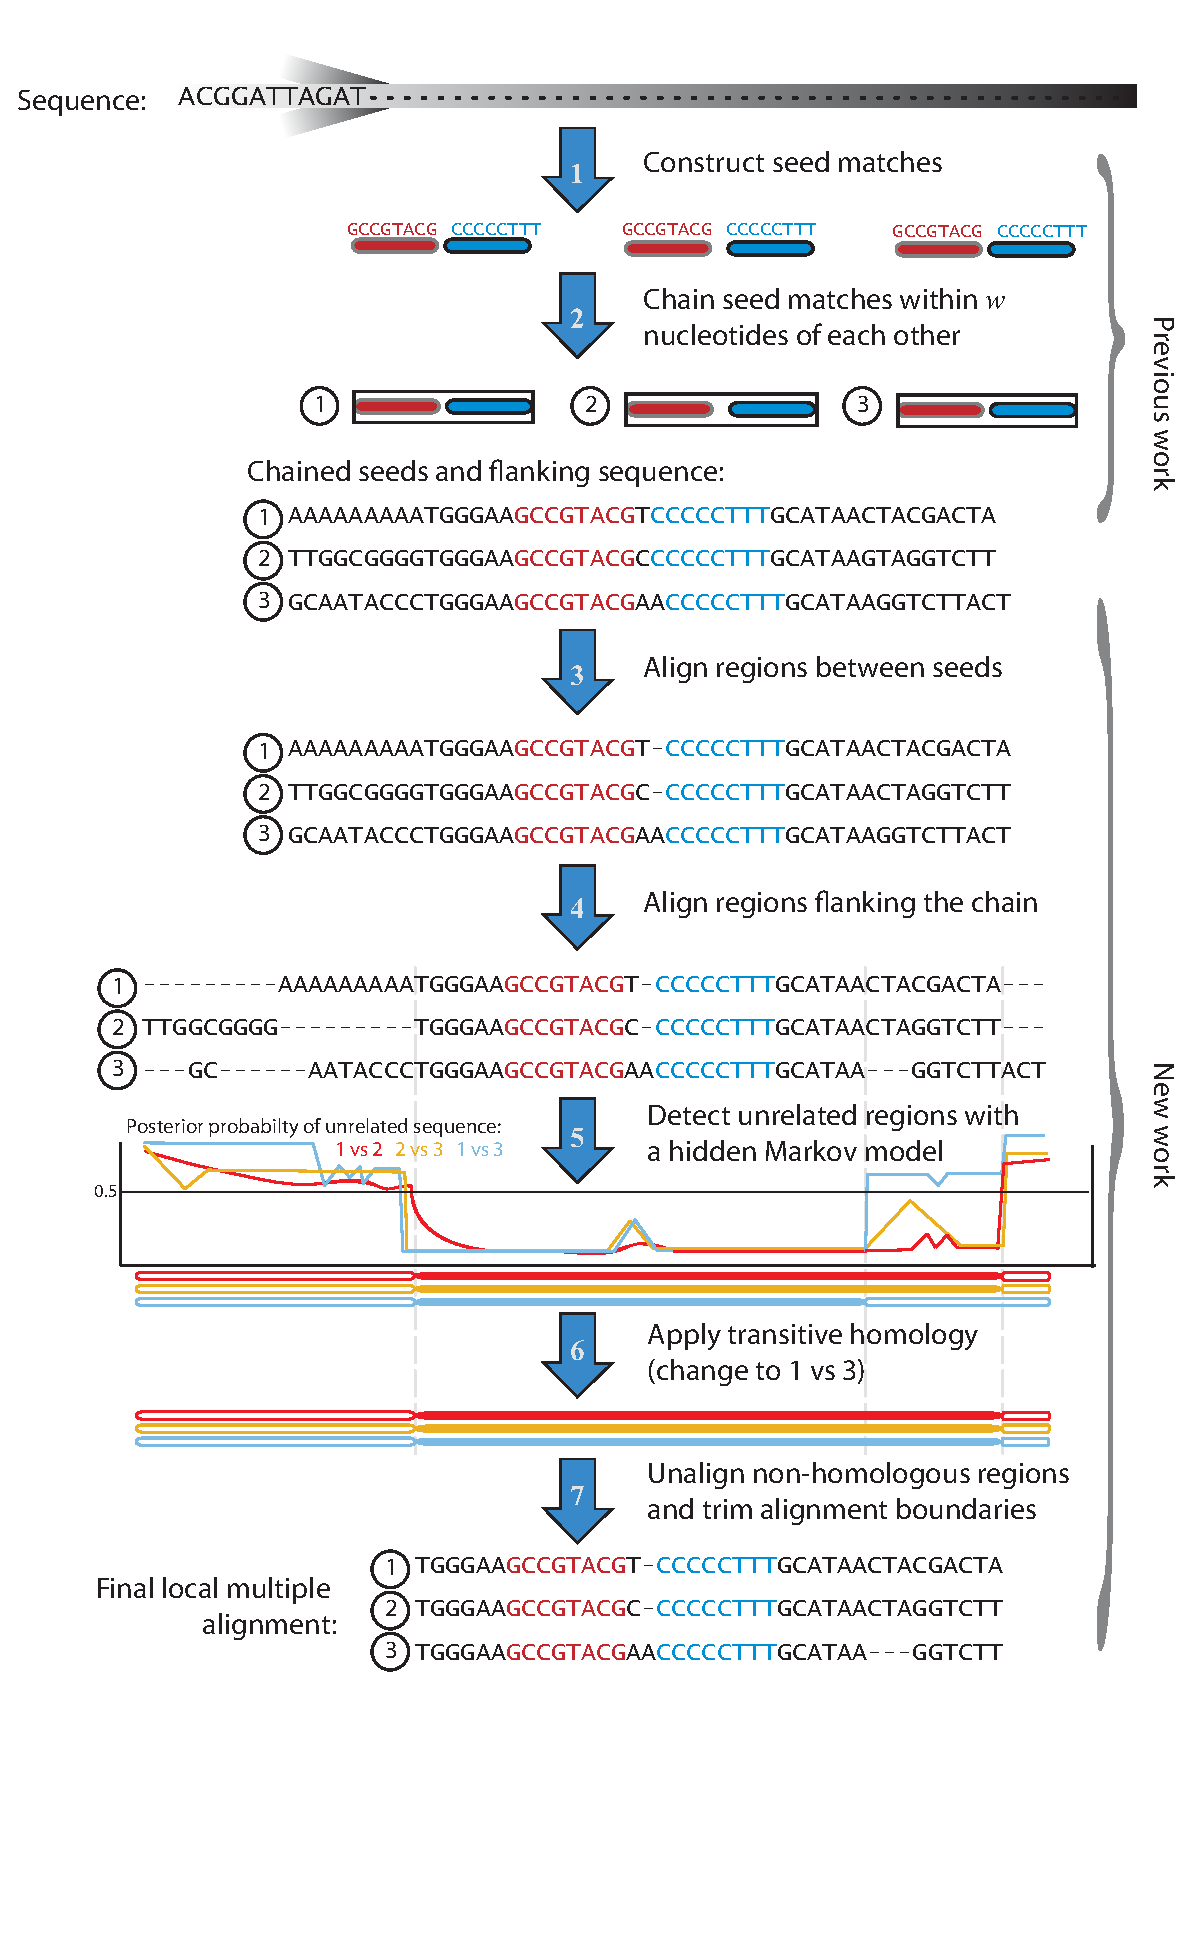
\epsfig{file=./figures/extension.eps,width=4.0in}
%\subfigure[Visual representation of our algorithm]{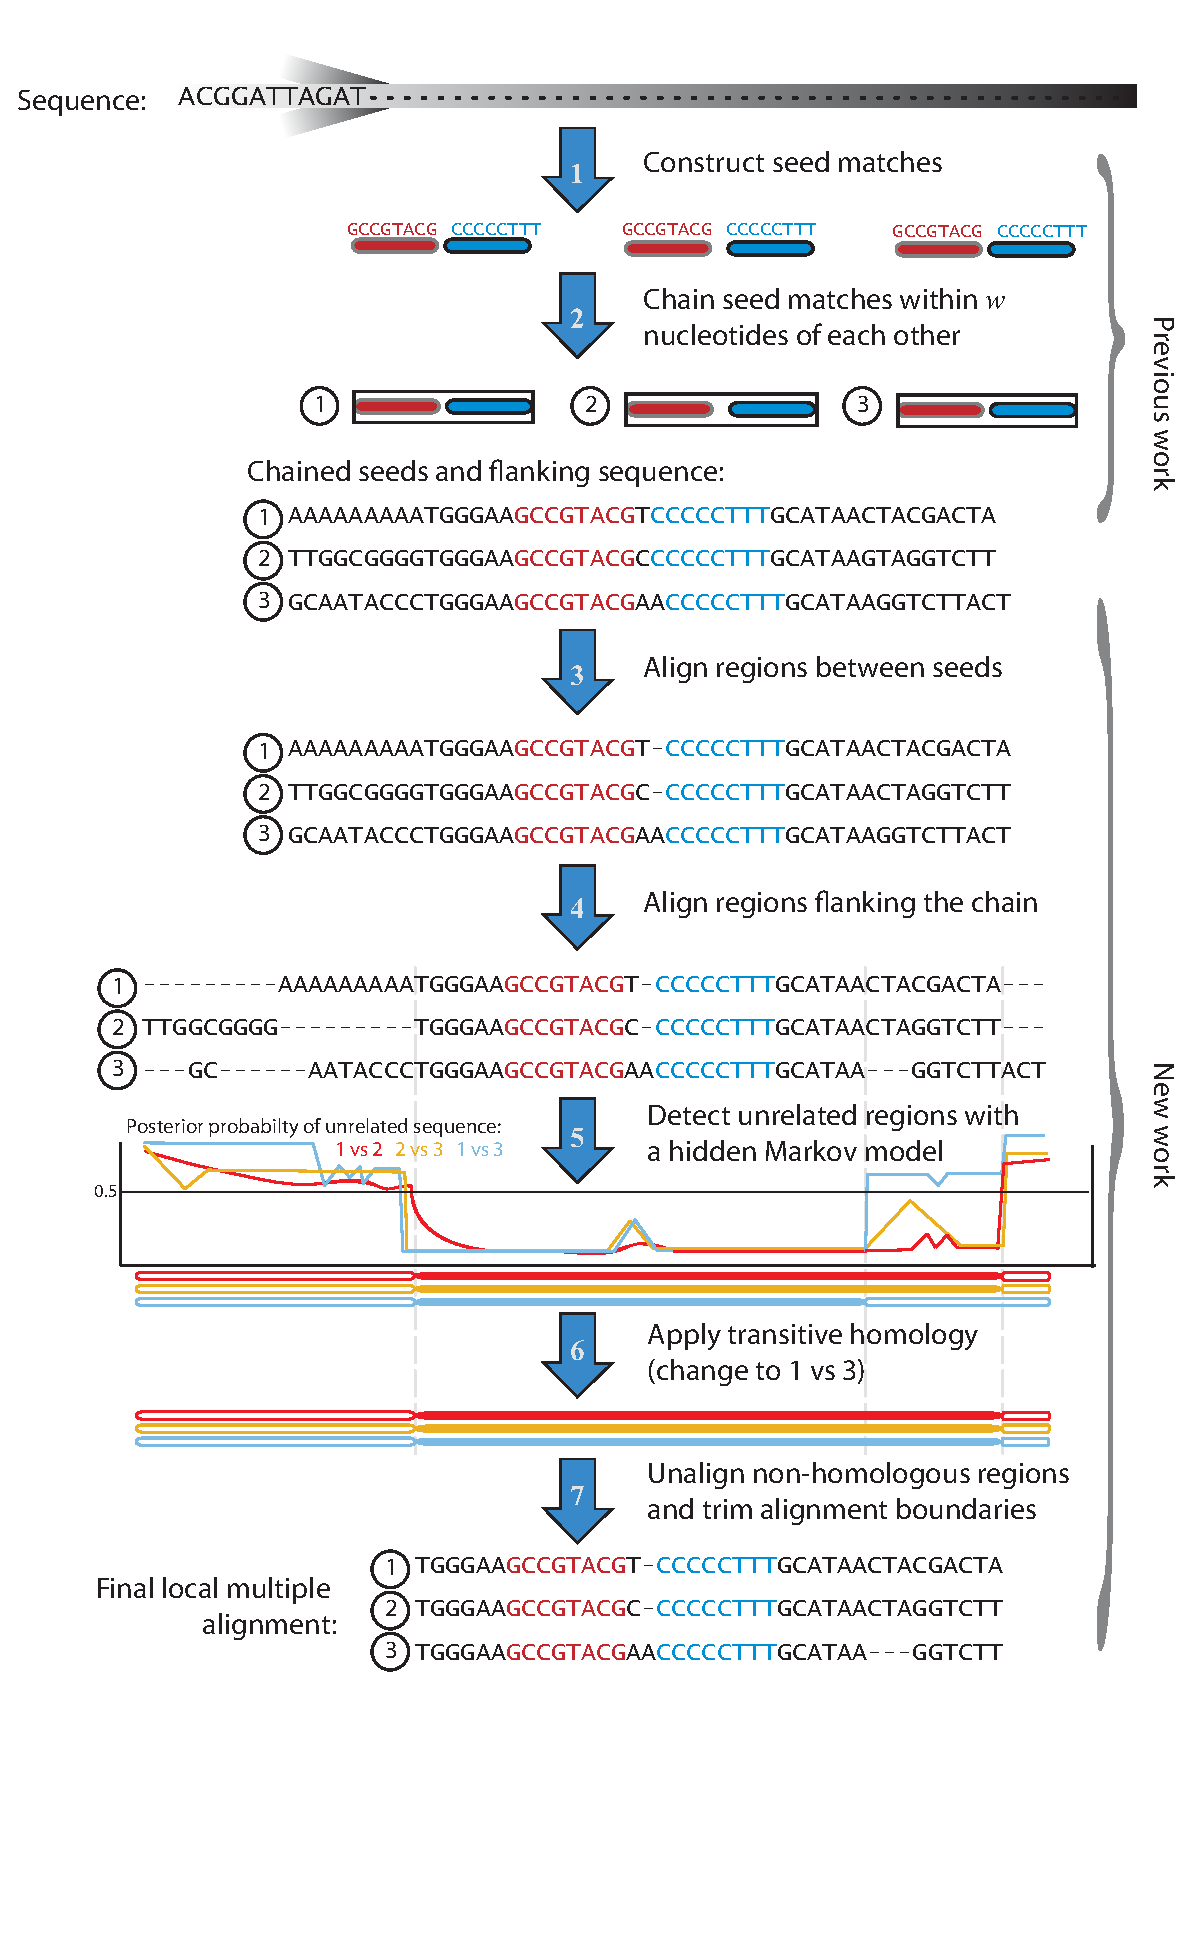
\epsfig{file=./figures/extension.eps,width=3.0in}}
%\subfigure[Flowchart of the algorithmic process ]{ 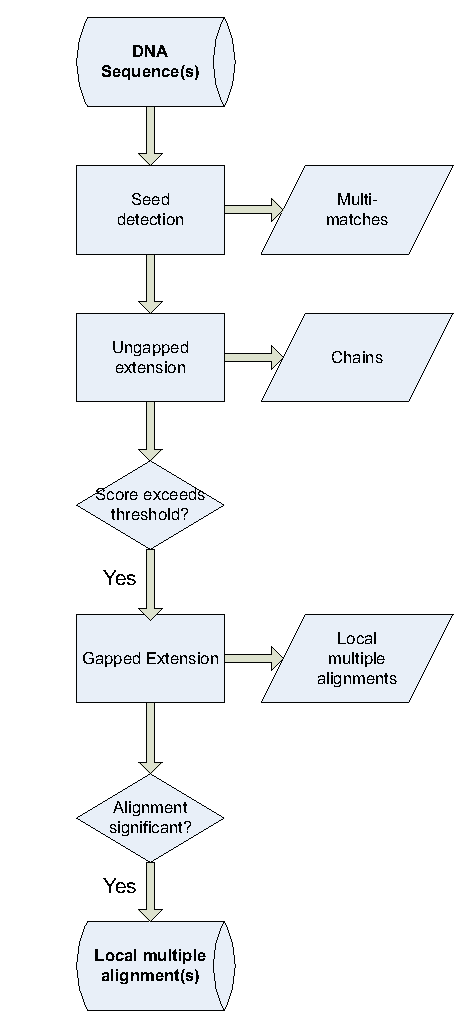
\epsfig{file=./figures/flowchart.eps,width=1.7in}}
\end{center}
\caption{Overview of the method, starting with an input sequence and ending with a set of local multiple alignments. First we (1) detect multi-matches in input sequence(s) using palindromic spaced seeds, then we perform (2) prioritized chaining of all multi-matches.  The resulting chain contains two matches and three match components labeled 1, 2, and 3.  We then perform gapped alignment of the region between chained matches (3).   In step (4), we perform a gapped extension by computing a global multiple alignment on the regions to the left and right of each chain component.  The resulting alignment may contain non-homologous sequence, so in step (5) we apply a Hidden Markov Model to detect the poorly aligned regions indicative of unrelated sequence.  In step (5), heavily diverged homologous sequences may be incorrectly classified as nonhomologous. The posterior probability of being in the non-homologous state for each alignment column is shown.  Step (6) computes transitive homology relationships to ensure a consistent alignment and aid detection of divergent homologous sequences.  Finally, in step (7) we unalign regions found to be non-homologous.  If we find after step (7) that the alignment boundaries have been extended, we acquire additional flanking sequence and return to step (4) for another round of extension.}
\label{fig-main}
\end{figure}


%\colorbox[named]{Gray}{adfa}

\subsection{Detecting seeds and multi-matches}

As a starting point for homology detection, we locate all spaced seeds of a given weight $z$ in the input sequence(s). The many advantages of using spaced seeds for sensitive homology detection have been well documented~\cite{ref-spacedseeds, ref-pattern}. The palindromic spaced seed pattern is analyzed at each position in the input sequence to identify all multi-matches.  Previously we have demonstrated that palindromic spaced seeds offer good efficiency and sensitivity on a variety of input sequences~\cite{ref-procrast}.

\subsection{Creating chains of multi-matches}

Once we have generated a list of multi-matches, we rely on our previously described method for efficiently filtration method for chaining ~\cite{ref-procrast}. A brief review of the method follows. In order to chain over each region of sequence $\mathcal{O}(1)$ times,
our method chains matches in order of decreasing multiplicity--we
extend the highest multiplicity matches first. We first chain all matches
with the same multiplicity within $w$
characters. When a match can no
longer be chained without including a gap larger than $w$
characters, our method identifies the neighboring \textit{subset}
matches within $w$ characters. We then \textit{link} each
neighboring subset match to the chained match. We refer to the
chained match as a \textit{superset} match. Rather than immediately
extend the subset match(es), we \textit{procrastinate} and extend
the subset match later when it has the highest multiplicity of any
match waiting to be extended. When chaining a match with a linked
superset, we immediately include the entire region covered by the linked superset
match--eliminating the need to re-examine sequence already covered by
a previous match extension.

\subsection{Gapped extension of high scoring chains}

Once we have finished the chaining process, we performed gapped alignment on all collinear regions located between two adjacent components to generate unextended local multiple alignments. We first evaluate the chain in order make a decision whether its worth spending computational resources on gapped extension. We can require that two seeds were present in the chain, allowing lower seed sizes $k$ to be used. This idea has been used in other local alignment heuristics~\cite{ref-blastz,ref-gappedblast,ref-blat} in order to minimize the number of gapped extensions that do not improve the boundaries of the chain.

To perform a gapped extension in each direction, we use MUSCLE to align the left/right region immediately surrounding the unextended local multiple alignments. The size of the extension window we send to MUSCLE is determined empirically to optimize efficiency and sensitivity. FIXME.
\subsubsection{Identifying non-homologous regions}
\begin{figure}[t]
\centering 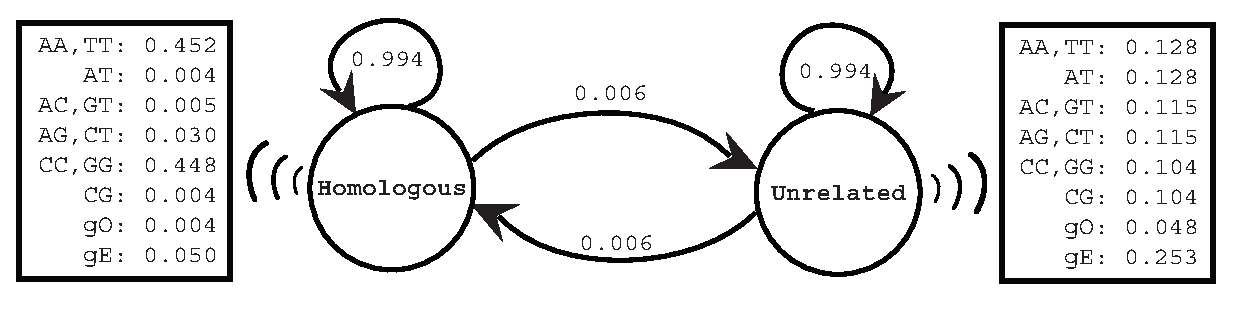
\epsfig{file=./figures/hmm.eps,width=3.5in}
\caption{HMM used to detect non-homologous sequence between two sequences x and y. gO stands for gap open, and gE gap extend. }

\label{fig-hmm}\vspace{-0.2cm}
\end{figure}

It often the case that the spaced seed approach is \emph{too} sensitive and does not always identify truly homologous sequence. This can cause non-homologous sequence to be aligned during gapped extension, since The MUSCLE alignment software dutifully reports the highest scoring global multiple alignment of input sequences, regardless of whether they are homologous or not. Since ideally we want to avoid aligning non-homologous sequence, especially when considering the consequences on downstream analysis, we need to identify any possible columns in the gapped extension that are likely to be non-Homologous. We have configured a Hidden Markov Model (Figure ~\ref{fig-hmm}) to do exactly this, consisting of two states, Homologous and Non-Homologous, to reject any column likely to be non-Homologous. Say something about HMM is constructed, how emission probabilities are extracted, how transmission probabilities were determined, and how homologous and nonhomologous states were decoded.

The emission probabilities were extracted from the HOXD substitution matrix presented in~\cite{hoxd}.

\begin{equation}
\begin{tabular}
{c|cccc}
& A & G & C & T \\
\hline
 A   & 91 & -114 &-31 & -123 \\
 G   & -114 & 100 &-125 & -31 \\
 C   & -31 & -125 &100 & -114\\
 T   & -123 & -31 &-114 & 91 \\
\end{tabular}
\end{equation}

\begin{equation}
s(x,y)= \log_{2}{\Bigg(\frac{p(x,y)}{q_{1}(x)q_{2}(x)}\Bigg)}
\end{equation}

Next, we calculated the gap open and gap extension emission probabilities empirically. To estimate the values in Non-homologous state we used a 10kb region taken from \emph{E. coli} CFT073 with 48\% GC content and its reverse (not complemented) and forced an alignment with MUSCLE.  We then counted the number of gap open and gap extend columns in the alignment of Non-homologous sequence. We found 483 and 2535 gap open and  gap extend columns, respectively.  For the homologous state the same procedure was used but this time we used an alignment of two relatively divergent(fixme:percentage?) homologous sequences with ~48\%GC, specifically \emph{Y. pestis} \& \emph{E. coli} k12(say, e. coli and yersinia). We found 44 and 507 gap open and  gap extend columns, respectively.  Since the values from the HOXD substitution matrix were calculated for ungapped alignments, we had to normalize the emission frequencies to account for the gap open and gap extension emission probabilities. All of the transmission and emission probabilities are reported in Figure~\ref{fig-hmm}.

Now that we have defined our probabilities for the model, we can defined the parameters for the HMM. We will refer to the sequence of hidden states (Homologous and Nonhomologous, henceforth H and N) as the path $\pi$. The $i$th state in the path is called $\pi_{i}$. The probability of the current state only depends on the previous state, and the transmission probability of $a_{kl}$ can be defined as follows:
\begin{equation}
a_{kl} = \textsl{P}\big(\pi_{i}=\textsl{l}\big|\pi_{i-i}=\textsl{k}\big).
\end{equation}

Similarly, we can define the emission probability that symbol $\textsl{b}$ is seen in state $\textsl{k}$ as:
\begin{equation}
e_{kb} = \textsl{P}\big(\pi_{i}=\textsl{b}\big|\pi_{i}=\textsl{k}\big).
\end{equation}
For our intents and purposes, the symbols in $\textsl{b}$ are simply all of the possible pairs in ${A,G,C,T,-}$ where order doesn't matter and neither does the strand (i.e. {\texttt AA=TT=AT=TA} ). Now we can define the join probability of observing a pairwise alignment $\textsl{A}$ and state sequence $\pi$:
\begin{equation}
\textsl{P}\big(\textsl{x},\pi\big) = a_{0\pi_{1}}\prod_{i=1}^\textsl{L}\textsl{e}_{\pi_{i}}(x_{i})\textsl{a}_{\pi_{i}\pi_{i+1}}.
\end{equation}
FIXME: Then, we decode the states $\pi$ $\textsl{P}(A |\pi)$ using the Viterbi algorithm~\cite{durbin}.


The result of applying a HMM to the alignment columns is a prediction of non-homologous segments among each pair of aligned sequences.  The remaining regions are predicted as homologous.  We apply transitivity to these homology predictions, resulting in a final set of consistent homology predictions.  See Figure~\ref{fig-main}, steps 5 and 6 for an example. Regions found to be non-homologous are unaligned from each other.

If have reached the end of the extension window without reaching a non-homologous state, we then improve our original seed boundaries and then trigger another round of chaining(and consequently another round of extension) in the same direction on the currently active, extend match. Else, we first determine if our chain boundaries have been improved, and then signal that we are done chaining/extending the current match in the current direction. If we have already processed the current chain in both directions, we stop entirely and proceed to the next multi-match in the priority queue.

\subsection{Assigning significance to local multiple alignments}
FIXME: insert statistics here!



\section{Results}


\subsection{Retrieval of randomly generated patterns}
%describe and present results(table)
%\begin{comment}

%\begin{table}[b]
%\scriptsize
%  \centering
%\begin{tabular}{|c|rcccc|}
%\hline Pattern & Program & Sn \% & Sp \% & T (s) & Sw \\
%\hline
%    & EulerAlign     &??? & ??? & 9 & - \\
%  1 & HomologMiner  &??? & ??? & 9 & - \\
%   &  procrastAlign  &??? & ??? & 9 & - \\
%
%\hline
%\end{tabular}
%\vspace{0.1cm}
% \label{tab-results}
%  \caption{}
%
%\end{table}

We have previously demonstrated the sensitivity of our chaining method in finding Alu repeats in
the human genome~\cite{ref-procrast}. Figure~\ref{fig-align} shows an example local multiple alignment of an ALU family as generated with \texttt{procrastAligner}. To highlight the benefits of our proposed heuristic for gapped extension, we compare \texttt{procrastAligner}'s performance to that of two related programs, EulerAlign~\cite{ref-related1} and HomologMiner~\cite{ref-homologminer}. For this comparison we have inserted mutated copies of randomly generated patterns into the complete genome of \emph{Mycoplasma genitalium}. \emph{M. genitalium} has been recognized as a complex and repeat rich genome, presenting a biologically relevant and challenging example to evaluate our method~\cite{ref-mycoplasma}. We generated and inserted DNA patterns into the genome as follows. To evaluate sensitivity and specificity of the methods as a function of multiplicity we generated 10 patterns for each multiplicity between 2 and 300. To generate each pattern, we first randomly determined a length for each multiplicity (larger pattern lengths for lower multiplicities and vice versa) using the following exponential equation: $l = 200e^{-0.01r}$ , where $r$ is pattern multiplicity and $l$ the calculated length. Next, we constructed the DNA pattern by using a background nucleotide frequency equivalent to the composition of \emph{Mycoplasma genitalium} ($A=0.34,T=0.34,G=0.16,C=0.16$). Then, we randomly mutated each copy of the pattern following a star tree topology. Some positions in the pattern were taken to be more likely to contain mutations by using a gamma-distributed rate heterogeneity. The distance between each mutation and length of indels were calculated using a Poisson distribution. Sequence divergence was varied from 0 substitutions per site (i.e. no divergence) to 1 substitution per site, allowing us also to analyze sensitivity and specificity of each method as a function of sequence divergence. Afterwards, we assigned an orientation to each copy by selecting either the forward or reverse strand.

Now that the pattern and all copies are ready to be inserted into the sequence, we randomly selected the minimum distance between any two copies (between 100-1000nt) following a uniform distribution and inserted each copy into the genome.  We started the analysis by simply recording each method's ability to recover all mutated copies of the  artificially generated pattern. If a copy of the pattern was found, it was recorded as a hit, else miss. We also used each method to find all significant multiple local alignments in the modified genome of \emph{M. genitalium} and recorded their respective sensitivity and specificity as a function of multiplicity and sequence divergences. Results of this experiment are reported in Table~\ref{tab-results}. Parameters used for each program were configured as follows: \\ \\ \textbf{procrastAligner}:\texttt{--z=9 --w=30 --solid=0 --chain=1 --extend=1}\\ \textbf{EulerAlign}:\texttt{ -k 9 -l -i 50 -v} \\ \textbf{HomologMiner}:\texttt{M=20 C=200 T=15 S=10}.

\subsection{144 HCV alignment? }
Next, we used a manually curated alignment of 144 Hepatitis C Virus sequences~\cite{ref-hcvdb} to analyze the
accuracy of our method.  We measure the
accuracy of our method as the fraction of pairwise
positions aligned in the correct alignment that are also present in
\texttt{procrastAligner} chains.  We measure positive predictive
value as the number of match component pairs that contain correctly
aligned positions out of the total number of match component pairs.


\begin{figure}[t]
\scriptsize
\begin{verbatim}
GATTGCTTGAACCTG--------GAGATTCAAGTGAGCTGAGATTGCACCACTGCATTCCAGCCTGGGC--AACAAAGCAAGACTCT
AATTGCTTGAACCTGGGAG-GCGGAGGTTGCAGTGAGCCGAGATGACGCCACTGCACTCCAGCCTGGGC--GACAGAGCA-------
AATCGCTTGAACCCAAGAGAGTGAAGGTTGCAGTGAGCTGAGATCATGCCACTTCACTCCAGCCTGAGTGAAACAGC----------
AATAACTTCAACCTGGGAG-ACAGAGGTTGCAGTCAGCTGAGATCGCACCACTGCATTCCAGCCTGGGT--GACAGACCGAGACTCT
AACTGCTTGAACTCGGGAG-GCAGAGATTGCAGTGAGCTGAGATCATGTCAATGCACTGCAGCTTGAGT--GACAGAGTG-------
AATCGCTTGAACCTGGGAG-GCAGAGGTTACAGAGAGCTGGGATTGTGCCACTGCACTCCGGCCTGGGC--AACAGAATG-------
AATCACTTGAACCTGGGAG-GCAGAGGTTACAGTGAGCCAAAATCGCGCCACTGCACTCCAACCTGGGC--AACACAGCAA------
AATTGCTTGAACCCGGGAG-GTGGAGGCTGCAGTGAGCCGAGATCATGCCACTGCACTCCAGCCT-GGT--GACAGAGCGAGA----
AATTGTTTGAACCCAGGAG-GCGGAGGCTGCAGTGAGCCGAGATTGTGTCACTGTACTCCAGCCTGGGCAAGACAGAG---------
AATCCCTTCAACCTGGGAA-ACAGAGGTTGCAGTGAGCCAAGATCGCACCATTGCACTCCAGTCTGGGC--AACAGAGAGA------
\end{verbatim}
\normalsize
\caption{Partial alignment of Alu-Sc subfamily found in \emph{H. sapiens} C1 esterase inhibitor gene. Each row represents an aligned ALU.}
\label{fig-align}
\end{figure}

\section{Discussion}

We have presented a sensitive and efficient heuristic for local multiple alignment.
We have extended previous results by converting chains of ungapped alignments into to multiple local alignments. We do so via a novel heuristic for directly computing local multiple alignments that utilizes the MUSCLE multiple alignment algorithm to compute gapped extensions of seed matches.  Our method assumes that a fixed number of nucleotides flanking a seed match is likely to be homologous and computes a global multiple alignment on the flanking region.  In some cases our assumption of flanking homology proves erroneous and results in an alignment of unrelated sequences.  We apply random walk statistics to detect any such non-homologous regions embedded in the global multiple alignment.
Present results have demonstrated both high sensitivity and specificity on aligning Alu
sequences and retrieving multiple copies of mutated patterns. We have also presented a statistic method for assigning significance to the resulting multiple local alignments that is used to select only the highly significant alignments.While we view the statistical significance proposal a preliminary, thus far the results of our significance assessment indicates a promising avenue of further research.

\section{Implementation}
We have implemented our method in a program, \texttt{procrastAligner}, available for Linux, Windows, and Mac OS X. Our open-source implementation is available as C++ source code licensed under the GPL. 

\section{ Acknowledgments }
AED was supported by NSF grant DBI-0630765. TJT was
supported by Spanish Ministry MECD Grant TIN2004-03382 and AGAUR
Training Grant FI-IQUC-2005.


\bibliographystyle{ws-procs9x6}
\bibliography{procrastination}

\end{document}
